\documentclass[conference]{IEEEtran}
\usepackage[utf8]{inputenc}
\usepackage[T1]{fontenc}
\usepackage[spanish]{babel}
\usepackage{graphicx}
\usepackage{booktabs}
\usepackage{array}
\usepackage{amsmath}
\usepackage{xcolor}
\usepackage{listings}
\usepackage{cite}
\usepackage{url}

\lstset{
  language=SQL,
  basicstyle=\ttfamily\fontsize{6.3}{7.3}\selectfont,
  keywordstyle=\bfseries,
  breaklines=true,
  breakatwhitespace=false,
  frame=single,
  columns=fullflexible,
  showstringspaces=false,
  literate={á}{{\'a}}1 {é}{{\'e}}1 {í}{{\'i}}1 {ó}{{\'o}}1 {ú}{{\'u}}1
           {Á}{{\'A}}1 {É}{{\'E}}1 {Í}{{\'I}}1 {Ó}{{\'O}}1 {Ú}{{\'U}}1
           {ñ}{{\~n}}1 {Ñ}{{\~N}}1 {¿}{{?`}}1 {¡}{{!`}}1,
  xleftmargin=1pt,
  xrightmargin=1pt,
  aboveskip=4pt,
  belowskip=2pt
}


% ---------------------------------------------------------------------------
% Capturas de Thunder Client recortadas (solo requiere main.tex).
% Se conserva la barra de la petición (método y URL) y, debajo, el estado, el
% tamaño, el tiempo y el cuerpo JSON de la respuesta. Se omite el panel de
% parámetros, que repite la URL y ocupaba casi la mitad de la imagen.
% Las capturas miden 1058 px de ancho: la barra de la petición ocupa los
% primeros 686 px y el panel de respuesta los últimos 368 px (1 px = 1 bp).
% Uso: \thunderclip{archivo}{alto en px de la captura}{ancho de la barra}
% La respuesta se dibuja con la misma escala que la barra.
\newcommand{\thunderclip}[3]{%
  \begin{tabular}[t]{@{}c@{}}
    \includegraphics[width=#3,trim=0bp \dimexpr#2bp-42bp\relax{} 372bp 0bp,clip]{#1}\\[1.5pt]
    \includegraphics[width=\dimexpr#3*368/686\relax,trim=690bp 0bp 0bp 0bp,clip]{#1}
  \end{tabular}}

\begin{document}

\title{Modelado relacional y análisis con SQL del conjunto de datos \emph{Streamers}}

\author{
\IEEEauthorblockN{Juan Sebastián García Valderrama}
\IEEEauthorblockA{Cód. 30000134625}
\and
\IEEEauthorblockN{Gabriela Rodríguez Lara}
\IEEEauthorblockA{Cód. 30000125720}
\and
\IEEEauthorblockN{John Alejandro Martin Galvis}
\IEEEauthorblockA{Cód. 30000090045}
\and
\IEEEauthorblockA{Facultad de Ingeniería, Universidad de San Buenaventura\\
Bogotá, Colombia\\
Laboratorio: Modelado y Análisis de Datos con SQL}
}

\maketitle

\begin{abstract}
Este informe describe cómo se transformó un archivo plano de 999 canales de transmisión en vivo y 17 columnas en un modelo relacional normalizado en MySQL, cómo se cargó mediante un programa en Node.js, cómo se explotó con consultas SQL orientadas a preguntas concretas y cómo esas consultas se expusieron mediante una API REST que se probó desde Visual Studio Code con la extensión Thunder Client. El hilo del trabajo es una decisión que se repite en cada etapa: conservar únicamente lo que el sistema necesita. Esa decisión determinó las columnas seleccionadas, la descomposición del grupo repetitivo de juegos en una tabla puente, el tratamiento de los valores faltantes y las ocho consultas finales. Los resultados muestran que \emph{Just Chatting} domina tanto como juego principal como secundario, que el español lidera el promedio de seguidores sin depender de unos pocos canales gigantes y que más días activos por semana no implican mayor audiencia promedio. En los casos comparados, las respuestas de la API coinciden con los resultados de las consultas SQL.
\end{abstract}

\begin{IEEEkeywords}
normalización, modelo entidad-relación, MySQL, Node.js, API REST, Thunder Client, consultas SQL, streamers.
\end{IEEEkeywords}

\section{Introducción}
El conjunto de datos asignado, \texttt{Streamers.csv}~\cite{dataset}, llega como una única tabla plana con un registro por canal y 17 columnas que mezclan identidad, idioma, juegos, audiencia y hábitos de transmisión. Una tabla así es cómoda para leer, pero incómoda para preguntar: por ejemplo, saber qué juegos aparecen en el dataset obliga a mirar dos columnas distintas, y cualquier cambio en un nombre repetido debe hacerse en cientos de filas.

El laboratorio~\cite{guia} pide descomponer esa tabla en lugar de trasladarla, justificar cada decisión y demostrar que el modelo resultante sirve para responder preguntas de análisis. Este informe sigue ese camino en el orden en que se tomaron las decisiones. Primero se define qué necesita el sistema y, a partir de eso, qué columnas se conservan (sección~II). Con esa información se construye el modelo y se normaliza paso a paso (sección~III), se implementa en MySQL (sección~IV) y se carga con un programa cuyo comportamiento se verifica (sección~V). Después se usa el modelo para responder cuatro consultas básicas (sección~VI) y las cuatro preguntas de análisis asignadas a este conjunto de datos (sección~VII). Finalmente se describe cómo esas consultas se expusieron mediante una API REST y se probaron desde Visual Studio Code con Thunder Client (sección~VIII).

\section{Del archivo plano a lo que el sistema necesita}
Las preguntas de análisis del laboratorio definen implícitamente el sistema: un repositorio de consulta de audiencias de canales de transmisión en vivo. Para responderlas, el sistema debe (R1) identificar cada canal con su idioma y tipo, (R2) registrar qué juegos transmite y en qué orden de preferencia, (R3) medir el tamaño de su audiencia, tanto acumulada (seguidores y vistas totales) como típica por transmisión (espectadores promedio), y (R4) conocer con qué frecuencia transmite. Cada columna se evaluó contra esos requisitos y no contra la limpieza del archivo: un campo puede ser perfectamente válido en el dataset original y aun así no tener ninguna función en este sistema.

La Tabla~\ref{tab:kept} resume las nueve columnas conservadas. La columna \texttt{TYPE} (personalidad o deportes electrónicos) no responde directamente a ninguna pregunta de análisis, pero se conserva porque distingue canales institucionales de creadores individuales, y esa distinción resultó indispensable para interpretar los promedios de audiencia (sección~VII-D).

\begin{table}[!t]
\caption{Columnas conservadas y requisito que las justifica}
\label{tab:kept}
\centering
\footnotesize
\begin{tabular}{@{}p{4.3cm}p{3.9cm}@{}}
\toprule
Columna del CSV & Requisito que atiende \\
\midrule
\texttt{NAME} & R1: identifica al canal (clave candidata) \\
\texttt{LANGUAGE} & R1: agrupar por idioma (consulta 2) \\
\texttt{TYPE} & R1: distinguir canales institucionales de individuales \\
{\scriptsize\texttt{MOST\_STREAMED\_GAME}}\newline{\scriptsize\texttt{2ND\_MOST\_STREAMED\_GAME}} & R2: juegos y orden de preferencia (consultas 1 y 3) \\
{\scriptsize\texttt{AVG\_VIEWERS\_PER\_STREAM}} & R3: audiencia típica por transmisión (consulta 4) \\
{\scriptsize\texttt{TOTAL\_FOLLOWERS}}\newline{\scriptsize\texttt{TOTAL\_VIEWS}} & R3: audiencia acumulada (consultas 2 y 3) \\
{\scriptsize\texttt{ACTIVE\_DAYS\_PER\_WEEK}} & R4: frecuencia de transmisión (consulta 4) \\
\bottomrule
\end{tabular}
\end{table}

Las ocho columnas restantes se excluyeron por las razones de la Tabla~\ref{tab:excluded}. Ninguna de las exclusiones se debe a que el dato esté sucio; todas se deben a que el sistema no tiene un requisito que las use.

\begin{table}[!t]
\caption{Columnas excluidas y justificación}
\label{tab:excluded}
\centering
\footnotesize
\begin{tabular}{@{}p{4.3cm}p{3.9cm}@{}}
\toprule
Columna & Justificación \\
\midrule
\texttt{RANK} & Atributo derivado: es la posición en un ordenamiento y se obtiene con \texttt{ORDER BY}. Almacenarlo crearía una inconsistencia en cuanto cambie cualquier medida. \\
{\scriptsize\texttt{AVERAGE\_STREAM\_DURATION}}\newline{\scriptsize\texttt{TOTAL\_TIME\_STREAMED}} & Describen el esfuerzo de transmisión en horas. El sistema mide frecuencia (R4), no duración. \\
{\scriptsize\texttt{FOLLOWERS\_GAINED\_PER\_STREAM}} & Métrica de crecimiento por transmisión; el sistema solo compara audiencias acumuladas (R3). \\
{\scriptsize\texttt{AVG\_GAMES\_PER\_STREAM}}\newline{\scriptsize\texttt{TOTAL\_GAMES\_STREAMED}} & Cuentan cuántos juegos usa un canal, pero no cuáles. El sistema necesita los juegos concretos (R2). \\
{\scriptsize\texttt{MOST\_ACTIVE\_DAY}}\newline{\scriptsize\texttt{DAY\_WITH\_MOST\_FOLLOWERS\_GAINED}} & Hábitos por día de la semana. Exigirían un catálogo de días que ninguna consulta usaría. \\
\bottomrule
\end{tabular}
\end{table}

\section{Modelo entidad-relación y normalización}
\subsection{Entidades y relaciones}
Siguiendo el modelo entidad-relación de Chen~\cite{chen76}, del archivo seleccionado se identifican cuatro entidades. \emph{Streamer} es la entidad principal. \emph{Idioma} y \emph{tipo de canal} son dominios de valores que se repiten (19 idiomas y 2 tipos en 999 canales). \emph{Juego} es la entidad que aparece en dos columnas. Un streamer habla exactamente un idioma y es de exactamente un tipo (relaciones N:1), pero puede transmitir varios juegos y un juego es transmitido por varios streamers (relación N:M), con un atributo propio de la relación: el orden de preferencia.

\subsection{Punto de partida}
Tras la selección de columnas, la relación de partida es
\begin{center}
\footnotesize
$R_0(\underline{\texttt{name}}, \texttt{language}, \texttt{type}, \texttt{main\_game}, \texttt{second\_game},$\\
$\texttt{avg\_viewers}, \texttt{total\_followers}, \texttt{total\_views}, \texttt{active\_days})$
\end{center}
La clave candidata es \texttt{name}: verificamos que los 999 nombres son distintos, y por tanto $\texttt{name} \rightarrow$ todos los demás atributos.

\subsection{Primera forma normal}
Un esquema está en primera forma normal cuando todos sus atributos son atómicos y no hay grupos repetitivos~\cite{codd70,elmasri16}. Los valores de $R_0$ son atómicos, pero \texttt{main\_game} y \texttt{second\_game} forman un grupo repetitivo: dos columnas del mismo dominio (juego) que solo se distinguen por una posición implícita en el nombre. Esto tiene consecuencias concretas. Preguntar \emph{qué juegos existen} o \emph{qué juego aparece más} exige combinar ambas columnas; un tercer juego requeriría modificar el esquema; y 77 canales tienen la segunda columna vacía, de modo que la ausencia de un dato se almacena como un valor nulo en una columna que en realidad es una lista.

La solución es mover el grupo repetitivo a su propia relación, con la posición convertida en un dato explícito. Resultan dos relaciones:
\begin{center}
\footnotesize
$R_1(\underline{\texttt{name}}, \texttt{language}, \texttt{type}, \texttt{avg\_viewers},$\\
$\texttt{total\_followers}, \texttt{total\_views}, \texttt{active\_days})$\\[2pt]
$R_2(\underline{\texttt{name}}, \underline{\texttt{preference\_order}}, \texttt{game})$
\end{center}
Con $R_2$, un canal sin segundo juego simplemente no tiene una segunda fila, y la relación N:M queda modelada mediante una tabla puente, como exige el caso~\cite{elmasri16}.

\subsection{Segunda forma normal}
La segunda forma normal exige que ningún atributo no clave dependa solo de una parte de la clave~\cite{codd72}. Esta etapa \textbf{no introduce cambios}, y por razones distintas en cada relación. En $R_1$ la clave tiene un solo atributo, así que una dependencia parcial es imposible por definición. En $R_2$ la clave es compuesta, pero el único atributo no clave (\texttt{game}) no queda determinado ni por \texttt{name} solo (un canal tiene dos juegos) ni por \texttt{preference\_order} solo (todos los canales tienen un juego en la posición 1); depende de la clave completa.

\subsection{Tercera forma normal}
La tercera forma normal prohíbe dependencias transitivas entre atributos no clave~\cite{codd72,kent83}. En $R_1$ ningún atributo descriptivo determina a otro: el idioma no determina el tipo ni las medidas de audiencia (hay canales de ambos tipos en varios idiomas), y las medidas son independientes entre sí. Estrictamente, el esquema ya cumple la tercera forma normal tras la primera.

Sin embargo, hay un problema de redundancia que la teoría de dependencias no detecta pero el dataset sí muestra: los mismos textos se repiten cientos de veces (\emph{English} en 401 filas, \emph{Just Chatting} en 412 apariciones). Esa repetición produce anomalías de actualización~\cite{elmasri16}, y el dataset ya contiene una: el mismo juego escrito de dos maneras (\emph{VALORANT} y \emph{Valorant}; \emph{Trackmania} y \emph{TrackMania}), que habría contado como juegos distintos. Por eso se descompone una vez más, extrayendo \texttt{language}, \texttt{streamer\_type} y \texttt{game} como tablas de catálogo referenciadas mediante claves foráneas. Esta es una decisión de diseño que va más allá de lo que exige estrictamente la tercera forma normal y se toma por integridad de los valores. El esquema final se muestra en la Fig.~\ref{fig:er}.

\begin{figure}[!htb]
\centering
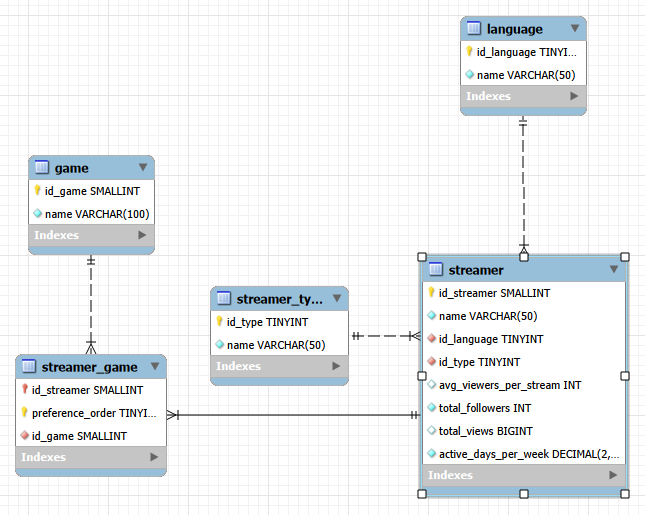
\includegraphics[width=\columnwidth]{figures/er_diagram.png}
\caption{Diagrama entidad-relación de la base de datos \texttt{db\_streamers}, obtenido con MySQL Workbench. La tabla puente \texttt{streamer\_game} resuelve la relación N:M entre canales y juegos.}
\label{fig:er}
\end{figure}

\section{Implementación del esquema}
El diagrama se tradujo a sentencias DDL para MySQL~\cite{mysql} que crean la base de datos \texttt{db\_streamers}. Los tipos se eligieron según los rangos observados en los datos: el máximo de seguidores (19\,000\,000) cabe en \texttt{INT UNSIGNED}, las vistas totales (hasta 572\,000\,000) se guardan en \texttt{BIGINT UNSIGNED} para tener holgura, y los días activos por semana en \texttt{DECIMAL(2,1)}, porque el archivo los reporta con un decimal. Las restricciones trasladan las reglas del modelo a la base de datos: claves únicas en los nombres de los catálogos y del canal, claves foráneas con \texttt{ON DELETE RESTRICT} hacia los catálogos y \texttt{CASCADE} desde la tabla puente, un \texttt{CHECK} que limita los días activos al intervalo 0--7, y en la tabla puente un \texttt{CHECK} que limita el orden a 1 o 2 y una clave única \texttt{(id\_streamer, id\_game)} que impide que un canal tenga el mismo juego como principal y como secundario. MySQL aplica las restricciones \texttt{CHECK} desde la versión 8.0.16~\cite{mysql}. El fragmento esencial es:

\begin{lstlisting}
-- Entidad principal: una fila por streamer
CREATE TABLE streamer (
  id_streamer SMALLINT UNSIGNED NOT NULL AUTO_INCREMENT,
  name VARCHAR(50) NOT NULL,
  id_language TINYINT UNSIGNED NOT NULL,
  id_type TINYINT UNSIGNED NOT NULL,
  -- NULL significa que la medición falta
  avg_viewers_per_stream INT UNSIGNED NULL,
  total_followers INT UNSIGNED NOT NULL,
  total_views BIGINT UNSIGNED NULL,
  active_days_per_week DECIMAL(2,1) NOT NULL,
  PRIMARY KEY (id_streamer),
  -- el nombre de un streamer no se puede repetir
  UNIQUE KEY uq_streamer_name (name),
  -- los días por semana van de 0 a 7
  CONSTRAINT ck_streamer_active_days
    CHECK (active_days_per_week BETWEEN 0 AND 7),
  -- idioma y tipo vienen de tablas de catálogo
  CONSTRAINT fk_streamer_language FOREIGN KEY
    (id_language) REFERENCES language (id_language),
  CONSTRAINT fk_streamer_type FOREIGN KEY
    (id_type) REFERENCES streamer_type (id_type)
);
-- Tabla puente: relación N:M entre streamer y game
CREATE TABLE streamer_game (
  id_streamer SMALLINT UNSIGNED NOT NULL,
  -- 1 = juego principal, 2 = segundo juego
  preference_order TINYINT UNSIGNED NOT NULL,
  id_game SMALLINT UNSIGNED NOT NULL,
  PRIMARY KEY (id_streamer, preference_order),
  -- un streamer no repite el mismo juego
  UNIQUE KEY uq_streamer_game (id_streamer, id_game),
  CHECK (preference_order IN (1, 2)), ...
);
\end{lstlisting}

Dos columnas, \texttt{avg\_viewers\_per\_stream} y \texttt{total\_views}, admiten \texttt{NULL}. La razón se explica en la sección siguiente.

\section{Programa de carga}
\subsection{Decisión arquitectónica}
El programa de carga es un \textbf{script independiente} en Node.js~\cite{nodejs}, no una aplicación por capas con rutas, controladores y servicios. La carga se ejecuta una sola vez, no expone una interfaz HTTP y su lógica no se reutiliza en ningún otro punto, de modo que las capas añadirían archivos sin añadir valor. La arquitectura por capas del proyecto se reserva para el otro consumidor de la base de datos: una API REST con Express~\cite{express}, organizada en rutas, controladores y capa de acceso a datos, que expone las consultas de análisis como \emph{endpoints}. Para que la ausencia de capas no vuelva ilegible el código, el script se divide en funciones pequeñas con una única responsabilidad: leer y validar el CSV con \texttt{csv-parse}~\cite{csvparse}, transformar los registros, insertar en el orden que exigen las claves foráneas (catálogos, canales y tabla puente) mediante \texttt{mysql2}~\cite{mysql2}, y verificar el resultado.

\subsection{Decisiones sobre la calidad de los datos}
Antes de insertar, el programa valida cada fila (campos obligatorios no vacíos, números válidos y dentro de rango). Si encuentra filas inválidas, aborta e informa cuáles son, en lugar de cargar parcialmente en silencio; existe un indicador opcional para omitirlas explícitamente. El análisis previo del archivo reveló cuatro situaciones que requirieron una decisión, todas registradas por el programa en su informe de salida (Tabla~\ref{tab:quality}).

\begin{table}[!t]
\caption{Decisiones de calidad de datos aplicadas en la carga}
\label{tab:quality}
\centering
\footnotesize
\begin{tabular}{@{}p{3.3cm}p{1.1cm}p{3.3cm}@{}}
\toprule
Situación & Filas & Decisión \\
\midrule
Espectadores promedio $=0$ & 120 & Cargar como \texttt{NULL} \\
Vistas totales $=0$ & 105 & Cargar como \texttt{NULL} \\
Sin juego secundario & 77 & No crear fila en \texttt{streamer\_game} \\
Juego secundario igual al principal & 6 & Omitir el secundario \\
Juego con distinta capitalización & 2 juegos & Unificar a la grafía más frecuente \\
\bottomrule
\end{tabular}
\end{table}

El valor $0$ en espectadores promedio y en vistas totales no es una medición real: canales con millones de seguidores no pueden promediar cero espectadores. Se interpreta como una medición ausente y se almacena como \texttt{NULL}, que es el mecanismo del modelo relacional para un valor desconocido o no disponible~\cite{elmasri16}. La consecuencia práctica es favorable: las funciones de agregación como \texttt{AVG} ignoran los \texttt{NULL}, de modo que los promedios no se contaminan con ceros falsos. Los 105 canales con vistas en cero son también canales con espectadores en cero; hay 15 más que solo tienen espectadores en cero.

Seis canales declaran el mismo juego como principal y como secundario (cinco coinciden literalmente y un sexto aparece al unificar la capitalización). Un segundo juego más transmitido no puede ser el primero, así que el dato es inconsistente y se omite la fila secundaria. Finalmente, \emph{VALORANT}/\emph{Valorant} y \emph{Trackmania}/\emph{TrackMania} se unificaron a la grafía más frecuente: el archivo contiene 213 cadenas distintas y el catálogo resultante tiene 211 juegos.

Quedan dos hallazgos que no se corrigieron porque no hay evidencia para hacerlo: 21 canales con vistas totales entre 1 y 999 (por ejemplo, 53 vistas para un canal con 4\,220\,000 seguidores, que probablemente es una unidad perdida) y 4 canales con 0 días activos, que pueden ser canales inactivos. Se conservan tal cual y se tienen en cuenta al interpretar resultados.

\subsection{Manejo de errores y verificación}
La carga ocurre dentro de una transacción con modo SQL estricto: cualquier violación de restricciones, tipo incompatible o valor fuera de rango produce un error en lugar de un ajuste silencioso, la transacción se revierte y el programa termina con código de salida distinto de cero, mostrando el código de error de MySQL y una pista de solución (por ejemplo, \texttt{ER\_ACCESS\_DENIED\_ERROR} indica credenciales incorrectas). Probamos dos fallos previsibles: ejecutar la carga con una contraseña incorrecta produce ese error, y ejecutarla por segunda vez sobre una base ya cargada se rechaza con un mensaje explícito en lugar de duplicar datos.

La verificación se hace dentro del propio programa, que compara el conteo esperado con el conteo real de cada tabla y falla si no coinciden. El resultado (Tabla~\ref{tab:counts}) es coherente: 999 canales, y $999-77-6=916$ segundos juegos, que sumados a los 999 principales dan las 1\,915 filas de la tabla puente.

\begin{table}[!t]
\caption{Verificación de la carga: filas por tabla}
\label{tab:counts}
\centering
\footnotesize
\begin{tabular}{@{}lrr@{}}
\toprule
Tabla & Esperadas & Insertadas \\
\midrule
\texttt{language} & 19 & 19 \\
\texttt{streamer\_type} & 2 & 2 \\
\texttt{game} & 211 & 211 \\
\texttt{streamer} & 999 & 999 \\
\texttt{streamer\_game} & 1\,915 & 1\,915 \\
\bottomrule
\end{tabular}
\end{table}

\section{Consultas básicas}
Con la base cargada y verificada, cada consulta se formula para responder una pregunta concreta y ninguna es un \texttt{SELECT *}. Las cuatro consultas básicas cubren los tipos exigidos: filtro con dos condiciones, \emph{join} de dos entidades, \emph{join} de cuatro entidades y agregación con \texttt{GROUP BY}.

\subsection{Filtro con dos condiciones}
\emph{¿Qué canales superan los 5 millones de seguidores y transmiten al menos cinco días a la semana?}
\begin{lstlisting}
-- Streamers grandes que además transmiten con frecuencia
SELECT streamer.name AS streamer_name,
       streamer.total_followers,
       streamer.active_days_per_week
FROM streamer
-- más de 5 millones de seguidores
WHERE streamer.total_followers > 5000000
  -- y al menos 5 días activos por semana
  AND streamer.active_days_per_week >= 5
ORDER BY streamer.total_followers DESC, streamer.name;
\end{lstlisting}
\begin{table}[!h]
\centering\footnotesize
\begin{tabular}{@{}lrr@{}}
\toprule
streamer\_name & total\_followers & active\_days \\
\midrule
auronplay & 16\,300\,000 & 5,0 \\
rubius & 15\,000\,000 & 5,0 \\
xqc & 12\,000\,000 & 6,3 \\
thegrefg & 11\,900\,000 & 6,3 \\
juansguarnizo & 11\,200\,000 & 5,5 \\
\multicolumn{3}{c}{\emph{(13 filas más)}} \\
\bottomrule
\end{tabular}
\end{table}
Solo 18 de los 999 canales (1,8\,\%) combinan una audiencia acumulada superior a 5 millones con una frecuencia de al menos cinco días semanales. La condición doble es lo que vuelve selectivo el filtro: una audiencia enorme no es frecuente en canales que transmiten pocos días, y la frecuencia alta no es habitual en canales muy grandes.

\subsection{\emph{Join} de dos entidades}
\emph{¿Quiénes son los diez canales con más seguidores y en qué idioma transmiten?}
\begin{lstlisting}
-- Top 10 de streamers por seguidores, con su idioma
SELECT streamer.name AS streamer_name,
       language.name AS language_name,
       streamer.total_followers
FROM streamer
-- el nombre del idioma está en la tabla de catálogo
INNER JOIN language
  ON language.id_language = streamer.id_language
ORDER BY streamer.total_followers DESC, streamer.name
LIMIT 10;
\end{lstlisting}
\begin{table}[!h]
\centering\footnotesize
\begin{tabular}{@{}lll@{}}
\toprule
streamer\_name & language\_name & total\_followers \\
\midrule
ninja & English & 19\,000\,000 \\
auronplay & Spanish & 16\,300\,000 \\
ibai & Spanish & 15\,600\,000 \\
rubius & Spanish & 15\,000\,000 \\
xqc & English & 12\,000\,000 \\
\multicolumn{3}{c}{\emph{(5 filas más)}} \\
\bottomrule
\end{tabular}
\end{table}
El \emph{join} es necesario porque el idioma ya no vive en la tabla del canal sino en el catálogo. Seis de los diez canales más seguidos transmiten en español y cuatro en inglés, aunque el español reúne solo 106 de los 999 canales (10,6\,\%). Esa sobrerrepresentación anticipa la pregunta de la sección~VII-B.

\subsection{\emph{Join} de cuatro entidades}
\emph{¿Cuál es el juego principal de los cinco canales en portugués con más seguidores?}
\begin{lstlisting}
-- Juego principal de los 5 streamers en portugués con más seguidores
SELECT streamer.name AS streamer_name,
       language.name AS language_name,
       game.name AS main_game,
       streamer.total_followers
FROM streamer
INNER JOIN language
  ON language.id_language = streamer.id_language
-- la tabla puente une los streamers con sus juegos
INNER JOIN streamer_game
  ON streamer_game.id_streamer = streamer.id_streamer
INNER JOIN game
  ON game.id_game = streamer_game.id_game
WHERE language.name = 'Portuguese'
  -- 1 = juego principal (2 sería el segundo juego)
  AND streamer_game.preference_order = 1
ORDER BY streamer.total_followers DESC, streamer.name
LIMIT 5;
\end{lstlisting}
\begin{table}[!h]
\centering\footnotesize
\begin{tabular}{@{}llr@{}}
\toprule
streamer\_name & main\_game & total\_followers \\
\midrule
alanzoka & Just Chatting & 7\,110\,000 \\
loud\_coringa & Grand Theft Auto V & 5\,380\,000 \\
gaules & Counter-Strike & 4\,139\,999 \\
casimito & Just Chatting & 3\,880\,000 \\
cellbit & Just Chatting & 3\,360\,000 \\
\bottomrule
\end{tabular}
\end{table}
La condición \texttt{preference\_order = 1} es una decisión del modelo y no un detalle: sin ella, cada canal aparecería dos veces, una por cada juego. Tres de los cinco canales brasileños más grandes tienen \emph{Just Chatting} como juego principal, un adelanto del liderazgo que se confirma en la sección~VII-A.

Esta misma unión de cuatro entidades se reutilizó en la API REST que se describe en la sección~\ref{sec:api}. La Fig.~\ref{fig:maingames} muestra la respuesta de \texttt{GET /streamers/main-games?limit=20}, que equivale a la consulta anterior sin el filtro de idioma y que, en lugar de ordenar por seguidores, lista los primeros 20 canales en orden alfabético. En los registros visibles se lee \texttt{2okos} con \emph{Just Chatting}, \texttt{39daph} con \emph{Art} y \texttt{4head} con \emph{Grand Theft Auto V}: una sola fila por canal, como exige la condición \texttt{preference\_order = 1}. La petición responde \texttt{200 OK} en 8~ms.

\begin{figure}[!t]
\centering
\thunderclip{figures/thunder/thunder_03_main_games.png}{405}{\columnwidth}
\caption{Prueba de \texttt{GET /streamers/main-games?limit=20}: juego principal de cada canal en orden alfabético (primeros registros).}
\label{fig:maingames}
\end{figure}

\subsection{Agregación con \texttt{GROUP BY}}
\emph{¿Cómo se comparan los canales de deportes electrónicos y los de personalidad en cantidad, seguidores promedio y días activos?}
\begin{lstlisting}
-- Comparación entre canales esports y personality
SELECT streamer_type.name AS streamer_type,
       COUNT(*) AS streamers,
       ROUND(AVG(streamer.total_followers)) AS avg_followers,
       ROUND(AVG(streamer.active_days_per_week), 2) AS avg_active_days
FROM streamer
INNER JOIN streamer_type
  ON streamer_type.id_type = streamer.id_type
-- una fila de resultado por cada tipo de streamer
GROUP BY streamer_type.id_type, streamer_type.name
ORDER BY streamers DESC;
\end{lstlisting}
\begin{table}[!h]
\centering\footnotesize
\begin{tabular}{@{}lrrr@{}}
\toprule
streamer\_type & streamers & avg\_followers & avg\_active\_days \\
\midrule
personality & 942 & 910\,444 & 3,66 \\
esports & 57 & 1\,067\,475 & 2,53 \\
\bottomrule
\end{tabular}
\end{table}
Los canales de deportes electrónicos son pocos (57 frente a 942), pero tienen un promedio de seguidores mayor y transmiten con menor frecuencia (2,53 días frente a 3,66). Es la primera señal de que los canales institucionales se comportan distinto de los individuales, una diferencia que se vuelve decisiva en la sección~VII-D. Esta misma agregación se expone como el \emph{endpoint} \texttt{/streamer-types/distribution}, cuya respuesta (57 canales \texttt{esports} y 942 \texttt{personality}) se muestra en la Fig.~\ref{fig:entorno}.

\section{Consultas de análisis}
\subsection{Juego principal y juego secundario}
\emph{¿Qué juego es el principal de más canales? ¿Coincide con el que más aparece como segunda opción?}
\begin{lstlisting}
-- Juegos elegidos con más frecuencia como juego principal
SELECT game.name AS game_name,
       COUNT(*) AS streamers_as_main_game
FROM streamer_game
INNER JOIN game ON game.id_game = streamer_game.id_game
-- 1 = juego principal
WHERE streamer_game.preference_order = 1
GROUP BY game.id_game, game.name
ORDER BY streamers_as_main_game DESC, game.name
LIMIT 5;
\end{lstlisting}
La segunda consulta es idéntica, con \texttt{preference\_order = 2} y el alias \texttt{streamers\_as\_second\_game}.
\begin{table}[!h]
\centering\footnotesize
\begin{tabular}{@{}lr@{\hspace{10pt}}lr@{}}
\toprule
\multicolumn{2}{c}{Principal} & \multicolumn{2}{c}{Secundario} \\
\midrule
Just Chatting & 257 & Just Chatting & 155 \\
League of Legends & 84 & VALORANT & 51 \\
Grand Theft Auto V & 74 & Minecraft & 42 \\
VALORANT & 63 & Grand Theft Auto V & 40 \\
Casino & 36 & Counter-Strike & 39 \\
\bottomrule
\end{tabular}
\end{table}
Sí coincide: \emph{Just Chatting} encabeza ambas listas, con 257 canales como juego principal (25,7\,\% de los 999) y 155 como segunda opción. Que un mismo valor domine los dos puestos sugiere que no es una preferencia dispersa sino una práctica estructural: \emph{Just Chatting} funciona más como una categoría de conversación que como un videojuego, y por eso sirve tanto de actividad central como de complemento. Fuera del primer puesto, las listas divergen. Los principales son títulos competitivos o de gran audiencia (\emph{League of Legends}, \emph{Grand Theft Auto V}, \emph{VALORANT}), mientras que \emph{Minecraft} aparece entre los tres más usados como segunda opción sin figurar entre los cinco principales: es un juego al que los canales recurren de forma complementaria más que como eje de su contenido.

La Fig.~\ref{fig:rankings} reproduce estos resultados desde la API. La misma ruta, \texttt{GET /games/rankings}, se llamó dos veces cambiando únicamente el parámetro \texttt{preferenceOrder}: con valor 1 devuelve los cinco juegos principales más frecuentes y con valor 2 los cinco más frecuentes como segunda opción. Las dos respuestas, de cinco objetos con \texttt{gameName} y \texttt{streamersCount}, coinciden cifra por cifra con la tabla de esta sección (por ejemplo, \emph{Just Chatting} con 257 y 155 canales) y tardan 6~ms cada una. Que un solo parámetro cambie el rol del juego sin modificar la consulta confirma que la tabla puente \texttt{streamer\_game} modela correctamente el orden de preferencia.

\begin{figure*}[!t]
\centering
\begin{minipage}[t]{0.485\textwidth}
\centering
\thunderclip{figures/thunder/thunder_06_rankings_main.png}{505}{\linewidth}\\[3pt]
{\footnotesize (a)}
\end{minipage}\hfill
\begin{minipage}[t]{0.485\textwidth}
\centering
\thunderclip{figures/thunder/thunder_07_rankings_second.png}{505}{\linewidth}\\[3pt]
{\footnotesize (b)}
\end{minipage}
\caption{Prueba de \texttt{GET /games/rankings}: (a) con \texttt{preferenceOrder=1} (juego principal) y \texttt{limit=5}; (b) con \texttt{preferenceOrder=2} (segundo juego) y el \texttt{limit} por defecto.}
\label{fig:rankings}
\end{figure*}

\subsection{Idioma con mayor promedio de seguidores}
\emph{¿Qué idioma agrupa el mayor promedio de seguidores por canal? ¿Es también el que tiene más canales o el liderazgo depende de pocos canales muy grandes?}
\begin{lstlisting}
-- Seguidores promedio por idioma, con y sin
-- el streamer más grande de cada idioma
SELECT language.name AS language_name,
  COUNT(*) AS streamers,
  ROUND(AVG(streamer.total_followers)) AS avg_followers,
  MAX(streamer.total_followers) AS max_followers,
  -- promedio sin el streamer más grande
  ROUND((SUM(streamer.total_followers)
    - MAX(streamer.total_followers))
    / NULLIF(COUNT(*) - 1, 0))
      AS avg_followers_without_top,
  -- porcentaje de seguidores que tiene el más grande
  ROUND(100 * MAX(streamer.total_followers)
    / SUM(streamer.total_followers), 1)
      AS top_streamer_share_pct
FROM streamer
INNER JOIN language
  ON language.id_language = streamer.id_language
GROUP BY language.id_language, language.name
ORDER BY avg_followers DESC, language.name;
\end{lstlisting}
\begin{table}[!h]
\caption{Idiomas por promedio de seguidores (selección)}
\centering\footnotesize
\begin{tabular}{@{}lrrrr@{}}
\toprule
Idioma & Canales & Prom. & Sin el mayor & \% del mayor \\
\midrule
Spanish & 106 & 1\,776\,154 & 1\,637\,831 & 8,7 \\
English & 401 & 1\,133\,737 & 1\,089\,071 & 4,2 \\
Turkish & 7 & 1\,094\,714 & 788\,833 & 38,2 \\
Portuguese & 82 & 775\,177 & 696\,969 & 11,2 \\
French & 72 & 766\,026 & 705\,970 & 9,1 \\
Russian & 115 & 442\,713 & 411\,948 & 7,8 \\
Czech & 3 & 343\,333 & 165\,000 & 68,0 \\
\bottomrule
\end{tabular}
\end{table}
El español tiene el mayor promedio (1\,776\,154 seguidores por canal), pero no es el idioma con más canales: el inglés tiene 401 frente a 106 y queda segundo en promedio. El liderazgo, por tanto, no proviene del volumen. Para saber si lo sostienen pocos canales gigantes, la consulta calcula el promedio sin el canal más grande de cada idioma. El del español apenas baja (de 1\,776\,154 a 1\,637\,831) y sigue siendo el más alto de todos, y su canal mayor aporta solo el 8,7\,\% de los seguidores del idioma. Su ventaja es, entonces, amplia y repartida. El caso contrario es el turco, que ocupa el tercer puesto con 1\,094\,714 pero cae a 788\,833 al retirar su mayor canal, que concentra el 38,2\,\% de la audiencia del idioma con solo siete canales. Los idiomas con muy pocos canales (checo, con tres, y el húngaro, el árabe y el rumano, con uno cada uno) no permiten conclusiones estadísticas, porque cualquier promedio sobre tan pocos datos lo determina un solo canal.

La Fig.~\ref{fig:languages} muestra la respuesta de \texttt{GET /languages/follower-stats}, que entrega por idioma la cantidad de canales, el promedio de seguidores, los seguidores del canal mayor y su porcentaje sobre el total del idioma. Las tres filas visibles coinciden con el Cuadro~V: el español con 106 canales, 1\,776\,154 seguidores promedio y un canal mayor de 16\,300\,000 (8,7\,\%); el inglés con 401, 1\,133\,737 y 4,2\,\%; y el turco con 7, 1\,094\,714 y 38,2\,\%. El \emph{endpoint} no devuelve el promedio sin el canal mayor, pero este se recupera con los campos que sí entrega: para el turco, $(7\times 1\,094\,714-2\,930\,000)/6 = 788\,833$, el mismo valor de la columna <<Sin el mayor>> del cuadro.

\begin{figure}[!t]
\centering
\thunderclip{figures/thunder/thunder_09_language_stats.png}{500}{\columnwidth}
\caption{Prueba de \texttt{GET /languages/follower-stats}: canales, seguidores promedio y porcentaje del canal mayor por idioma (español, inglés y turco).}
\label{fig:languages}
\end{figure}

\subsection{Juego principal de un canal que es secundario de otro}
\emph{¿Existen canales cuyo juego principal es el secundario de otro canal? ¿Qué relación hay entre ellos en seguidores o vistas?}
\begin{lstlisting}
-- Streamers cuyo juego principal es también el segundo
-- juego de otro streamer
SELECT COUNT(DISTINCT main_link.id_streamer)
         AS streamers_with_shared_main_game,
       COUNT(DISTINCT main_link.id_game) AS games_shared
FROM streamer_game AS main_link
-- main_link = filas de juegos principales
WHERE main_link.preference_order = 1
  -- otro streamer tiene ese juego como segundo juego
  AND EXISTS (
    SELECT 1
    FROM streamer_game AS second_link
    WHERE second_link.preference_order = 2
      AND second_link.id_game = main_link.id_game
      AND second_link.id_streamer <> main_link.id_streamer);
\end{lstlisting}
\begin{lstlisting}
-- Seguidores y vistas según el rol de los juegos compartidos
SELECT streamer_game.preference_order AS game_role,
       COUNT(*) AS streamer_game_links,
       ROUND(AVG(streamer.total_followers)) AS avg_followers,
       -- AVG ignora las vistas NULL
       ROUND(AVG(streamer.total_views)) AS avg_total_views,
       COUNT(streamer.total_views) AS links_with_views_data
FROM streamer_game
INNER JOIN streamer
  ON streamer.id_streamer = streamer_game.id_streamer
-- solo juegos usados como principal y como secundario
WHERE streamer_game.id_game IN
        (SELECT id_game FROM streamer_game
         WHERE preference_order = 1)
  AND streamer_game.id_game IN
        (SELECT id_game FROM streamer_game
         WHERE preference_order = 2)
GROUP BY streamer_game.preference_order
ORDER BY streamer_game.preference_order;
\end{lstlisting}
La primera consulta responde la existencia: 934 de los 999 canales (93,5\,\%) tienen como juego principal uno que otro canal usa como secundario, y hay 70 juegos en esa situación de los 211 del catálogo. La respuesta es afirmativa, pero casi trivial: con una oferta tan concentrada en pocos juegos populares, la coincidencia es lo esperable. Lo informativo es la relación entre ambos grupos, que se calcula con la segunda consulta sobre los 70 juegos compartidos.

La Fig.~\ref{fig:shared} confirma la primera cifra desde la API: \texttt{GET /streamers/main-game-shared-as-secondary} responde \texttt{200 OK} con el objeto \texttt{\{"streamersCount": 934\}}. Como la respuesta es un único número (22 bytes, 7~ms), la comprobación es directa: el valor coincide con el de la primera consulta.

\begin{figure}[!t]
\centering
\thunderclip{figures/thunder/thunder_05_shared_secondary.png}{150}{\columnwidth}
\caption{Prueba de \texttt{GET /streamers/main-game-shared-as-secondary}: 934 canales tienen como principal un juego que es secundario de otro canal.}
\label{fig:shared}
\end{figure}
\begin{table}[!h]
\centering\footnotesize
\begin{tabular}{@{}lrrr@{}}
\toprule
Rol del juego & Filas & Prom. seguidores & Prom. vistas totales \\
\midrule
Principal (1) & 934 & 941\,822 & 34\,032\,115 \\
Secundario (2) & 746 & 1\,040\,064 & 35\,031\,815 \\
\bottomrule
\end{tabular}
\end{table}
Los canales que tienen esos juegos como secundarios son, en promedio, ligeramente mayores: 10,4\,\% más seguidores y 2,9\,\% más vistas totales (las vistas excluyen los valores nulos: 832 y 706 filas con dato). La diferencia es pequeña, y una tercera consulta que desagrega los cinco juegos con más filas muestra que no es un patrón consistente: en \emph{League of Legends} (833\,169 frente a 1\,411\,014 seguidores), \emph{Grand Theft Auto V} (815\,434 frente a 1\,070\,768) y \emph{VALORANT} (675\,278 frente a 1\,012\,396) los canales con ese juego como secundario son mayores, pero en \emph{Just Chatting} (1\,271\,079 frente a 1\,130\,277) y \emph{Fortnite} (2\,802\,486 frente a 1\,782\,544) ocurre lo contrario.

La Fig.~\ref{fig:comparison} muestra el \emph{endpoint} \texttt{GET /games/preference-comparison}, que devuelve para cada juego la cantidad de canales y los promedios de seguidores y de vistas totales, tanto como juego principal como secundario. Los dos primeros registros coinciden con las cifras anteriores: \emph{Just Chatting} aparece en 257 canales como principal y 155 como secundario, con 1\,271\,079 y 1\,130\,277 seguidores promedio, y \emph{League of Legends} en 84 y 36 canales, con 833\,169 y 1\,411\,014. La respuesta añade las vistas totales promedio, y estas no siguen el mismo sentido que los seguidores: \emph{Just Chatting} tiene más seguidores como principal pero más vistas como secundario (30\,144\,545 frente a 29\,758\,214), y \emph{League of Legends} muestra el patrón contrario, con más seguidores como secundario pero más vistas como principal (54\,601\,548 frente a 41\,227\,172). Incluso para un mismo juego, entonces, las dos medidas de audiencia no apuntan en la misma dirección.

\begin{figure}[!t]
\centering
\thunderclip{figures/thunder/thunder_08_preference_comparison.png}{440}{\columnwidth}
\caption{Prueba de \texttt{GET /games/preference-comparison?limit=15}: cantidad de canales, seguidores promedio y vistas promedio de cada juego como principal y como secundario (primeros registros).}
\label{fig:comparison}
\end{figure}

No hay entonces una relación sistemática entre el rol del juego y el tamaño del canal. Una hipótesis plausible, que estos datos no permiten probar, es que los canales grandes diversifican hacia juegos competitivos como segunda opción, mientras que en los juegos de conversación o de moda los grandes los usan como eje.

\subsection{Días activos por semana y audiencia}
\emph{Agrupando los canales por rango de días activos por semana, ¿qué rango tiene el mejor promedio de espectadores por transmisión? ¿Más días activos implica más audiencia?}
\begin{lstlisting}
-- Espectadores promedio por rango de días activos por semana
SELECT CASE
         WHEN streamer.active_days_per_week < 2 THEN '0 to <2 days'
         WHEN streamer.active_days_per_week < 4 THEN '2 to <4 days'
         WHEN streamer.active_days_per_week < 6 THEN '4 to <6 days'
         ELSE '6 to 7 days'
       END AS active_days_range,
       COUNT(*) AS streamers,
       -- streamers que sí tienen dato de espectadores (no NULL)
       COUNT(streamer.avg_viewers_per_stream)
         AS streamers_with_viewer_data,
       ROUND(AVG(streamer.avg_viewers_per_stream))
         AS avg_viewers_per_stream
FROM streamer
GROUP BY active_days_range
ORDER BY MIN(streamer.active_days_per_week);
\end{lstlisting}
\begin{table}[!h]
\centering\footnotesize
\begin{tabular}{@{}lrrr@{}}
\toprule
Rango (días) & Canales & Con dato & Prom. espectadores \\
\midrule
0 a $<$2 & 222 & 156 & 30\,976 \\
2 a $<$4 & 305 & 277 & 20\,489 \\
4 a $<$6 & 373 & 355 & 18\,492 \\
6 a 7 & 99 & 91 & 27\,505 \\
\bottomrule
\end{tabular}
\end{table}
A primera vista, el mejor rango es el de menos días (0 a menos de 2, con 30\,976 espectadores promedio) y la relación no es monótona: baja hasta el rango de 4 a 6 días y vuelve a subir en el de 6 a 7. Una correlación de Pearson calculada en SQL con las medidas de dispersión poblacional,
\begin{lstlisting}
-- Correlación de Pearson: días activos vs espectadores promedio
SELECT COUNT(*) AS streamers_with_viewer_data,
  ROUND((AVG(streamer.active_days_per_week
        * streamer.avg_viewers_per_stream)
   - AVG(streamer.active_days_per_week)
     * AVG(streamer.avg_viewers_per_stream))
   / (STDDEV_POP(streamer.active_days_per_week)
     * STDDEV_POP(streamer.avg_viewers_per_stream)),
  3) AS pearson_r
FROM streamer
-- ignora los streamers sin dato de espectadores
WHERE streamer.avg_viewers_per_stream IS NOT NULL;
\end{lstlisting}
da $r=-0{,}074$ con 879 canales: prácticamente no hay relación lineal. Por tanto, más días activos \emph{no} implican mayor audiencia promedio. Sin embargo, el resultado agregado esconde un efecto de composición que conviene comprobar. Los canales institucionales del primer rango pueden estar inflando el promedio, así que se repite el cálculo separando por tipo de canal (consulta A4c del repositorio, que agrupa por rango y por \texttt{streamer\_type}).
\begin{table}[!h]
\caption{Espectadores promedio por rango y tipo de canal}
\centering\footnotesize
\begin{tabular}{@{}lrrrr@{}}
\toprule
Rango (días) & \multicolumn{2}{c}{personality} & \multicolumn{2}{c}{esports} \\
 & Canales & Prom. & Canales & Prom. \\
\midrule
0 a $<$2 & 197 & 17\,835 & 25 & 99\,833 \\
2 a $<$4 & 285 & 13\,127 & 20 & 115\,090 \\
4 a $<$6 & 366 & 17\,790 & 7 & 53\,397 \\
6 a 7 & 94 & 23\,348 & 5 & 99\,006 \\
\bottomrule
\end{tabular}
\end{table}
Los canales de deportes electrónicos promedian entre 53\,397 y 115\,090 espectadores, de cinco a ocho veces más que los de personalidad, y 25 de ellos caen en el primer rango, es decir, el 11\,\% de ese grupo. Ese puñado de canales explica por qué el primer rango gana en el promedio global. Si se consideran solo los canales de personalidad, el mejor rango es el de 6 a 7 días (23\,348), aunque la relación sigue sin ser monótona (el rango de 2 a 4 días es el más bajo, con 13\,127). Además, el rango de menos días tiene la mayor proporción de datos faltantes (66 de 222 canales, 29,7\,\%, frente a menos del 10\,\% en los demás), por lo que su promedio global descansa en menos canales. En conclusión, el rango de 0 a 2 días tiene el mejor promedio, pero por la composición del grupo y no porque transmitir poco atraiga más público, y la frecuencia de transmisión por sí sola es un mal predictor de la audiencia.

\section{API REST y pruebas con Thunder Client}
\label{sec:api}
Además de los scripts SQL, las consultas se expusieron como \emph{endpoints} de una API REST en Node.js, de modo que cada pregunta de análisis se pueda consultar con una petición HTTP. Esta sección describe el entorno en que se hicieron las pruebas, los \emph{endpoints} disponibles y cómo se contrastaron sus respuestas con las consultas SQL de las secciones~VI y~VII.

\subsection{Entorno de pruebas}
Las pruebas y consultas del laboratorio se realizaron en Visual Studio Code~\cite{vscode}, conectado a un servidor Node.js~\cite{nodejs} con Express~\cite{express} que consulta la base \texttt{db\_streamers} mediante \texttt{mysql2}~\cite{mysql2}, y con la extensión Thunder Client~\cite{thunder} para enviar las peticiones HTTP y revisar las respuestas. El procedimiento fue directo. Primero se instalaron las dependencias con \texttt{npm install} y se definió la contraseña de MySQL en la variable de entorno \texttt{DB\_PASSWORD} de la terminal, de modo que nunca queda guardada en el repositorio. Luego \texttt{npm start} inició el servidor, que imprime \texttt{Server running in http://localhost:5000} (Fig.~\ref{fig:servidor}). Desde Thunder Client se creó una petición \texttt{GET} por \emph{endpoint}, con sus parámetros, y en cada una se revisaron el estado, el tamaño, el tiempo y el cuerpo JSON de la respuesta.
El proyecto sigue la arquitectura por capas descrita en la sección~V-A: su carpeta contiene \texttt{constants}, \texttt{controllers}, \texttt{dao}, \texttt{env}, \texttt{middlewares}, \texttt{routes}, \texttt{services}, \texttt{utils} y \texttt{server.js}. La Fig.~\ref{fig:entorno} muestra la primera prueba desde Thunder Client: una petición \texttt{GET} a \texttt{/streamer-types/distribution} que responde \texttt{200 OK} en 5~ms con la cantidad de canales de cada tipo.

\begin{figure}[!t]
\centering
\begin{tabular}[t]{@{}c@{}}
  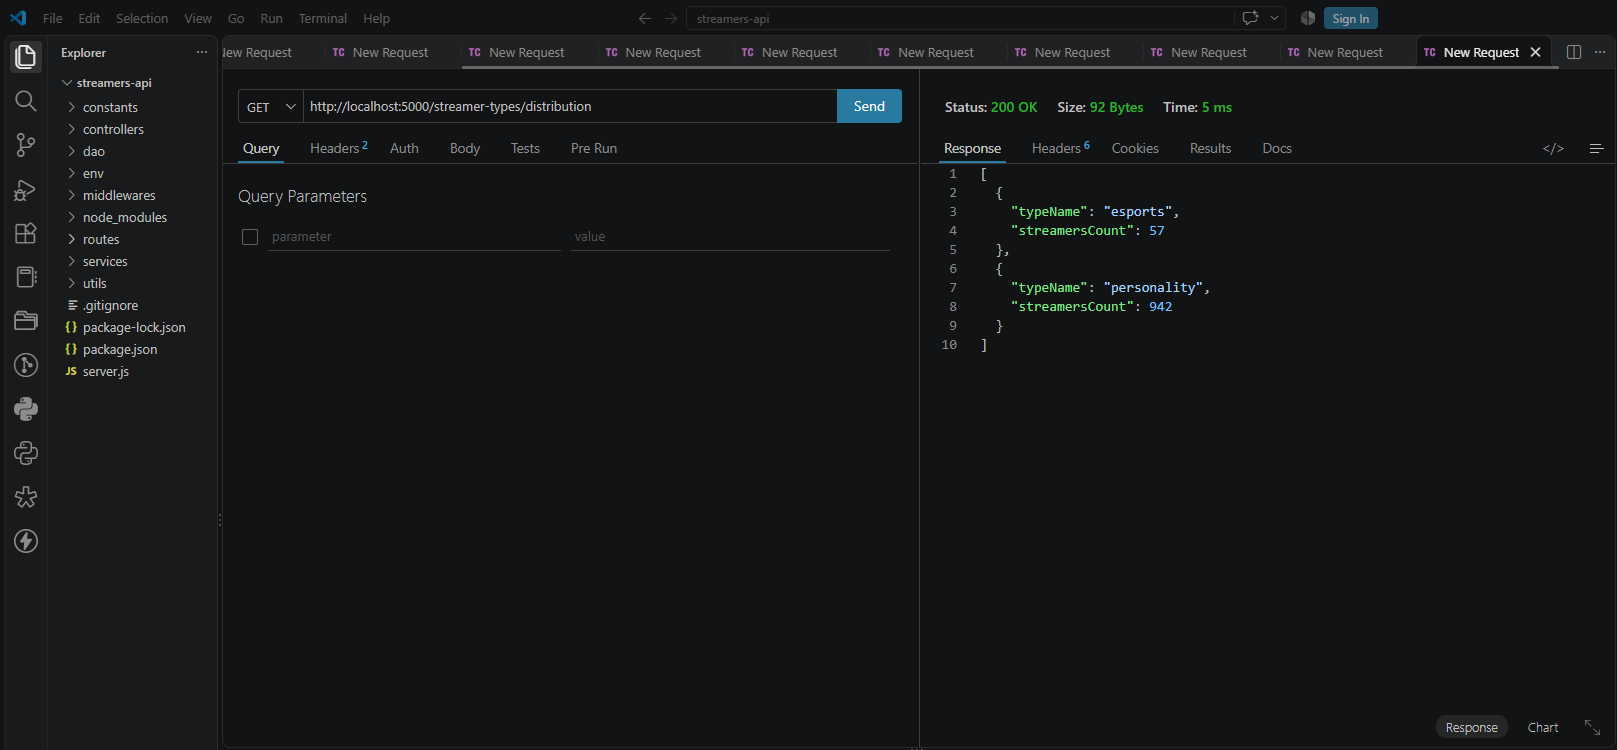
\includegraphics[width=\columnwidth,trim=228bp 625bp 705bp 82bp,clip]{figures/thunder/thunder_01_entorno.png}\\[1.5pt]
  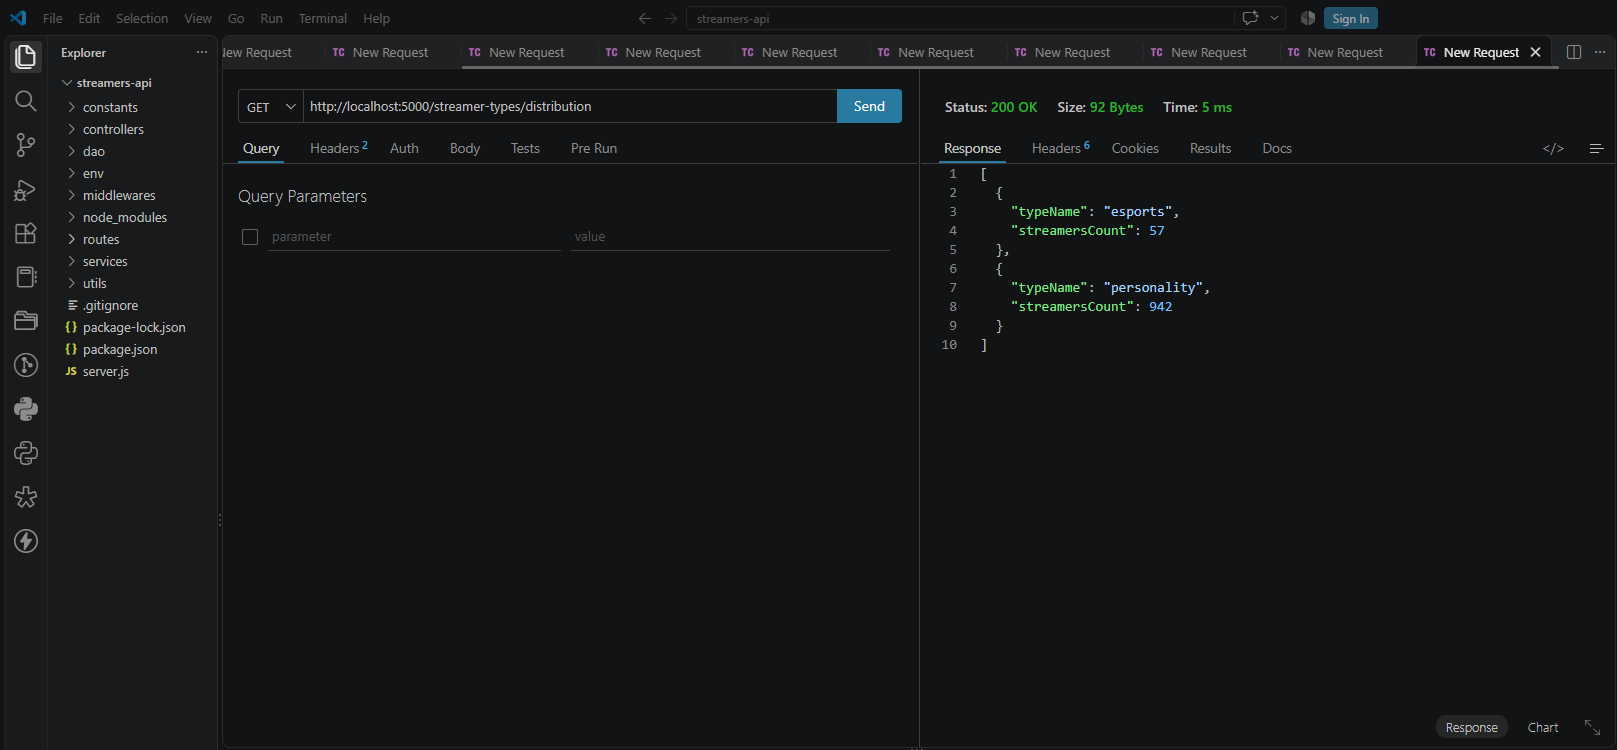
\includegraphics[width=\dimexpr\columnwidth*368/684\relax,trim=922bp 388bp 327bp 84bp,clip]{figures/thunder/thunder_01_entorno.png}
\end{tabular}
\caption{Prueba de \texttt{GET /streamer-types/distribution}: cantidad de canales por tipo (\texttt{esports} y \texttt{personality}).}
\label{fig:entorno}
\end{figure}

\begin{figure}[!t]
\centering

\includegraphics[width=0.7\columnwidth,trim=0 0 370 5,clip]{figures/thunder/thunder_02_servidor.png}
\caption{Servidor Express iniciado con \texttt{npm start} en la terminal de Visual Studio Code.}
\label{fig:servidor}
\end{figure}

\subsection{\emph{Endpoints} expuestos}
La Tabla~\ref{tab:endpoints} lista los nueve \emph{endpoints} (todos \texttt{GET}), los parámetros que aceptan con su valor por defecto y la consulta del informe con la que se relacionan. Los parámetros se validan en un \emph{middleware} antes de llegar al controlador: \texttt{limit} debe ser un entero entre 1 y 100, \texttt{preferenceOrder} vale 1 o 2 y \texttt{minActiveDays} es un número entre 0 y 7. Un valor inválido produce el estado 400, una ruta inexistente el 404 y un fallo de la base de datos el 500, siempre con cuerpo JSON.

\begin{table*}[!t]
\caption{Endpoints de la API y consulta del informe con la que se relacionan}
\label{tab:endpoints}
\centering
\footnotesize
\setlength{\tabcolsep}{3pt}
\begin{tabular}{@{}p{6.8cm}p{3.8cm}p{4.7cm}p{1.7cm}@{}}
\toprule
\emph{Endpoint} & Parámetros (por defecto) & Relación con el informe & Captura \\
\midrule
\texttt{/streamers} & \texttt{minActiveDays} (5), \texttt{limit} (10) & Canales con más espectadores promedio (adicional) & --- \\
\texttt{/streamers/main-games} & \texttt{limit} (20) & Juego principal de cada canal (ampliación de VI-C) & Fig.~\ref{fig:maingames} \\
\texttt{/streamers/views-per-follower} & \texttt{limit} (10) & Vistas totales por seguidor (adicional) & Fig.~\ref{fig:viewsper} \\
\texttt{/streamers/main-game-shared-as-secondary} & --- & VII-C: existencia de juegos compartidos & Fig.~\ref{fig:shared} \\
\texttt{/streamers/activity-ranges} & --- & VII-D: audiencia por rango de días activos & --- \\
\texttt{/games/rankings} & \texttt{preferenceOrder} (1), \texttt{limit} (5) & VII-A: juegos principales y secundarios & Fig.~\ref{fig:rankings} \\
\texttt{/games/preference-comparison} & \texttt{limit} (15) & VII-C: seguidores y vistas por rol del juego & Fig.~\ref{fig:comparison} \\
\texttt{/languages/follower-stats} & --- & VII-B: seguidores promedio por idioma & Fig.~\ref{fig:languages} \\
\texttt{/streamer-types/distribution} & --- & VI-D: canales por tipo & Fig.~\ref{fig:entorno} \\
\bottomrule
\end{tabular}
\end{table*}

\subsection{Resultados y contraste con las consultas SQL}
Cada petición de la Tabla~\ref{tab:endpoints} con captura respondió \texttt{200 OK} en menos de 10~ms. En los cinco \emph{endpoints} que tienen una consulta equivalente en las secciones~VI y~VII, las cifras devueltas por la API coinciden con las de esas consultas. Por eso las capturas de cuatro de ellos se presentaron junto a la consulta que reproducen: el ranking de juegos (Fig.~\ref{fig:rankings}, sección~VII-A), las estadísticas por idioma (Fig.~\ref{fig:languages}, sección~VII-B) y, en la sección~VII-C, la existencia de juegos compartidos (Fig.~\ref{fig:shared}) y la comparación por rol (Fig.~\ref{fig:comparison}). El quinto, la distribución por tipo, es el de la Fig.~\ref{fig:entorno}.

El contraste cifra por cifra es el siguiente. Con \texttt{preferenceOrder=1} y con \texttt{preferenceOrder=2}, la API devuelve las dos listas de la sección~VII-A, con \emph{Just Chatting} a la cabeza en ambas (257 y 155 canales). La comparación por rol reproduce la desagregación de la sección~VII-C para \emph{Just Chatting} y \emph{League of Legends}, y esa inversión de signo entre ambos juegos es la misma que se interpretó en el análisis SQL. Las estadísticas por idioma repiten el Cuadro~V: el español encabeza con 106 canales y 1\,776\,154 seguidores promedio, y su canal mayor aporta solo el 8,7\,\% del idioma, mientras que el turco (7 canales, 1\,094\,714) concentra el 38,2\,\% en su canal mayor. La diferencia es que el \emph{endpoint} devuelve los seguidores del canal mayor y su porcentaje, pero no el promedio sin ese canal, que solo calcula la consulta SQL. Los dos últimos \emph{endpoints} con equivalente son numéricos: la respuesta \texttt{\{"streamersCount": 934\}} es el mismo valor de la sección~VII-C (934 de 999 canales comparten su juego principal con la lista de secundarios de otro canal), y la distribución por tipo (Fig.~\ref{fig:entorno}) devuelve 57 canales \texttt{esports} y 942 \texttt{personality}, igual que la agregación de la sección~VI-D.

Los otros dos \emph{endpoints} probados no tienen una consulta equivalente en el informe. \texttt{/streamers/main-games} (Fig.~\ref{fig:maingames}) es la consulta de cuatro entidades de la sección~VI-C sin el filtro de idioma, y se explicó allí. \texttt{/streamers/views-per-follower} (Fig.~\ref{fig:viewsper}) ordena los canales por vistas totales divididas entre seguidores: encabezan \texttt{nba2kleague} (810,1), \texttt{xop0} (538,7), \texttt{uzra} (437,5) y \texttt{att} (423,5), canales de entre 20\,400 y 240\,000 seguidores con muchas vistas acumuladas. En las capturas largas Thunder Client muestra solo los primeros registros de la respuesta.

\begin{figure}[!t]
\centering
\thunderclip{figures/thunder/thunder_04_views_per_follower.png}{445}{\columnwidth}
\caption{Prueba de \texttt{GET /streamers/views-per-follower?limit=10}: vistas totales por seguidor, de mayor a menor (primeros registros).}
\label{fig:viewsper}
\end{figure}

\section{Conclusiones}
La decisión que organizó todo el trabajo fue conservar solo lo que el sistema necesita. De ella se derivó la selección de nueve columnas, la identificación del grupo repetitivo de juegos como el único problema real de normalización y su resolución con una tabla puente, y la extracción de catálogos que evitó contar como distintos juegos escritos de dos maneras. También quedó claro que la tercera forma normal, estrictamente, no obligaba a cambios en este dataset, y que los catálogos responden a una necesidad de integridad y no de la teoría de dependencias.

Los resultados de análisis muestran un patrón común: los promedios globales se explican mejor cuando se examina quién los compone. El español lidera el promedio de seguidores por una ventaja amplia y no por un canal gigante; el primer rango de días activos gana por la presencia de canales institucionales; y la relación entre el rol de un juego y el tamaño de los canales cambia de signo de un juego a otro. Las conclusiones están limitadas por la calidad de los datos: 120 canales sin espectadores promedio, 21 valores de vistas totales sospechosamente bajos y varios idiomas con uno a tres canales. Además, el conjunto es una fotografía en un momento dado, de modo que las relaciones encontradas son descriptivas y no causales. Por último, las consultas también se expusieron mediante una API REST en Node.js y se probaron desde Visual Studio Code con Thunder Client: en los cinco \emph{endpoints} con una consulta equivalente, las respuestas coincidieron con los resultados de las secciones~VI y~VII, lo que confirma que la capa de acceso a datos reproduce fielmente las consultas SQL. El código (incluida la API que expone las consultas de análisis), el script DDL, las consultas y las capturas de las pruebas están disponibles en el repositorio~\cite{repo}.

\begin{thebibliography}{99}
\bibitem{dataset} ``Streamers.csv,'' conjunto de datos asignado en el laboratorio, Facultad de Ingeniería, Universidad de San Buenaventura, Bogotá, Colombia, 2026.
\bibitem{guia} S. A. Reyes Gómez, ``Laboratorio: Modelado y Análisis de Datos con SQL,'' guía de laboratorio, Facultad de Ingeniería, Universidad de San Buenaventura, Bogotá, Colombia, 2026.
\bibitem{chen76} P. P.-S. Chen, ``The entity-relationship model---Toward a unified view of data,'' \emph{ACM Trans. Database Syst.}, vol. 1, no. 1, pp. 9--36, Mar. 1976.
\bibitem{codd70} E. F. Codd, ``A relational model of data for large shared data banks,'' \emph{Commun. ACM}, vol. 13, no. 6, pp. 377--387, Jun. 1970.
\bibitem{elmasri16} R. Elmasri and S. B. Navathe, \emph{Fundamentals of Database Systems}, 7th ed. Hoboken, NJ, USA: Pearson, 2016.
\bibitem{codd72} E. F. Codd, ``Further normalization of the data base relational model,'' in \emph{Data Base Systems}, R. Rustin, Ed. Englewood Cliffs, NJ, USA: Prentice-Hall, 1972, pp. 33--64.
\bibitem{kent83} W. Kent, ``A simple guide to five normal forms in relational database theory,'' \emph{Commun. ACM}, vol. 26, no. 2, pp. 120--125, Feb. 1983.
\bibitem{mysql} Oracle Corporation, ``MySQL 8.0 Reference Manual.'' [Online]. Available: \url{https://dev.mysql.com/doc/refman/8.0/en/} (accessed Oct. 10, 2026).
\bibitem{nodejs} OpenJS Foundation, ``Node.js documentation.'' [Online]. Available: \url{https://nodejs.org/docs/latest/api/} (accessed Oct. 10, 2026).
\bibitem{express} ``Express: Fast, unopinionated, minimalist web framework for Node.js.'' [Online]. Available: \url{https://expressjs.com/} (accessed Oct. 10, 2026).
\bibitem{csvparse} ``CSV Parse.'' [Online]. Available: \url{https://csv.js.org/parse/} (accessed Oct. 10, 2026).
\bibitem{mysql2} ``mysql2: MySQL client for Node.js.'' GitHub. [Online]. Available: \url{https://github.com/sidorares/node-mysql2} (accessed Oct. 10, 2026).
\bibitem{vscode} Microsoft, ``Documentation for Visual Studio Code.'' [Online]. Available: \url{https://code.visualstudio.com/docs} (accessed Oct. 11, 2026).
\bibitem{thunder} Thunder Client Limited, ``Thunder Client: API testing tool for VS Code.'' [Online]. Available: \url{https://www.thunderclient.com/} (accessed Oct. 11, 2026).
\bibitem{repo} J. S. García Valderrama, G. Rodríguez Lara, and J. A. Martin Galvis, ``streamers-sql-lab,'' GitHub repository, 2026. [Online]. Available: \url{https://github.com/USUARIO/streamers-sql-lab}
\end{thebibliography}

\end{document}
